Para a análise da solução desenvolvida e identificação de problemas foram feitos
testes variados. Este capítulo foi dividido em seções que representam as
descobertas mais relevantes ao longo da pesquisa e desenvolvimento. A
Seção~\ref{sec:extracao_da_placa_resultados} vai descrever os resultados obtidos
na experimentação com a extração da placa e dos caracteres nas imagens. São os casos
onde o algoritmo detectou a presença de um carro e identificou uma placa. A
Seção~\ref{sec:reconhecimento_dos_caracteres_resultados} vai abordar os
resultados obtidos no reconhecimento dos caracteres, avaliar se a placa e caracteres
extraídos foram lidos corretamente. Por fim, a
Seção~\ref{sec:performance_resultados} vai abordar como performa o algoritmo no
sistema embarcado no computador \emph{Raspberry Pi}.

Foram coletadas imagens de 48 veículos distintos para analisar a capacidade de
reconhecimento do sistema. A tabela~\ref{tab:resultados} mostra o número de
imagens processadas, o número de imagens onde a placa foi encontrada com sucesso
e o número de imagens onde foi possível reconhecer o valor da placa corretamente.
Existe uma diferença entre os casos onde não foi possível detectar uma placa e os
casos onde foi possível mas ela foi detectada erroneamente. No segundo há um falso
positivo, identificando um veículo que não estava no local.

\begin{table}[]
\centering
\caption{Resultados obtidos}
\label{tab:resultados}
\begin{tabular}{@{}lr@{}}
\toprule
Placas                               & \multicolumn{1}{l}{Resultado} \\ \midrule
Total de Imagens                     & 48                           \\
Imagens onde a placa foi encontrada  & 22                            \\
Imagens onde a placa foi reconhecida corretamente & 19
\end{tabular}
\end{table}

\section{Extração da placa e caracteres}
\label{sec:extracao_da_placa_resultados}

Das 48 imagens adquiridas, apenas em 22 imagens foi possível extrair a placa e os caracteres. Dessas 48 imagens, 27 foram adquiridas ao ar livre, durante o dia e 21 foram adquiridas em local fechado, com iluminação baixa. Com essa diferenças foi possível analisar o sistema nos dois tipos de ambientes. Nas imagens ao ar livre, com boa iluminação, houve um percentual de 55\% de acerto, enquanto nas imagens em ambiente fechado, com baixa iluminação, houve um percentual de acerto de 33\%. Os resultados comparativos podem ser vistos na Tabela~\ref{tab:resultados_ambientes}. Os exemplos são poucos para tirar conclusões, mas indicam que pode existir mais dificuldade para reconhecer placas em imagens mais escuras.

\begin{table}[]
\centering
\caption{Resultados obtidos em diferentes ambientes}
\label{tab:resultados_ambientes}
\begin{tabular}{@{}lr@{}}
\toprule
Placas                                      		& \multicolumn{1}{l}{Resultado} \\ \midrule
Imagens ao ar livre com boa iluminação     			& 27                            \\
Total de acertos com boa iluminação    			 	& 15                            \\
Percentual de acertos com boa iluminação    		 & 55\%                            \\
Imagens em ambiente fechado com baixa iluminação     & 21                            \\
Total de acertos com baixa iluminação    			 & 7                            \\
Percentual de acertos com baixa iluminação 			& 33\%
\end{tabular}
\end{table}

O algoritmo de extração da placa é limitado com relação a distância que o carro
está na imagem. Na etapa de abertura e fechamento morfológicos, que tem o
objetivo de detectar as áreas de placas candidatas, o tamanho do elemento
estruturante influencia diretamente a qualidade da extração. Se utilizado um
elemento estruturante muito grande, é possível que na etapa de abertura, a placa
seja erodida junto com o ruído. Se utilizado um elemento estruturante muito
pequeno, muitas regiões sobram, diminuindo a performance do reconhecimento.

Outro problema foi observado na extração de placas de carros cuja cor da lataria
é muito semelhante à cor da placa. Carros de cor prata ou branco são maioria nos casos
em que a placa não foi encontrada. Isso ocorre pois, na fase de limiarização, não foi 
possível dividir o tom da lataria e da placa em grupos diferentes. Foram feitos testes
utilizando limiarização adaptativa para comparar os resultados, mas ela obteve menos sucesso
que utilizando limiar global, em geral. Detalhes significativos de cores diferentes também dificultam
a extração. Na Figura~\ref{fig:peugeot_gay} há um exemplo de veículo que o sistema teve dificuldade
de reconhecer por estes motivos.

\begin{figure}[H]
	\centering
	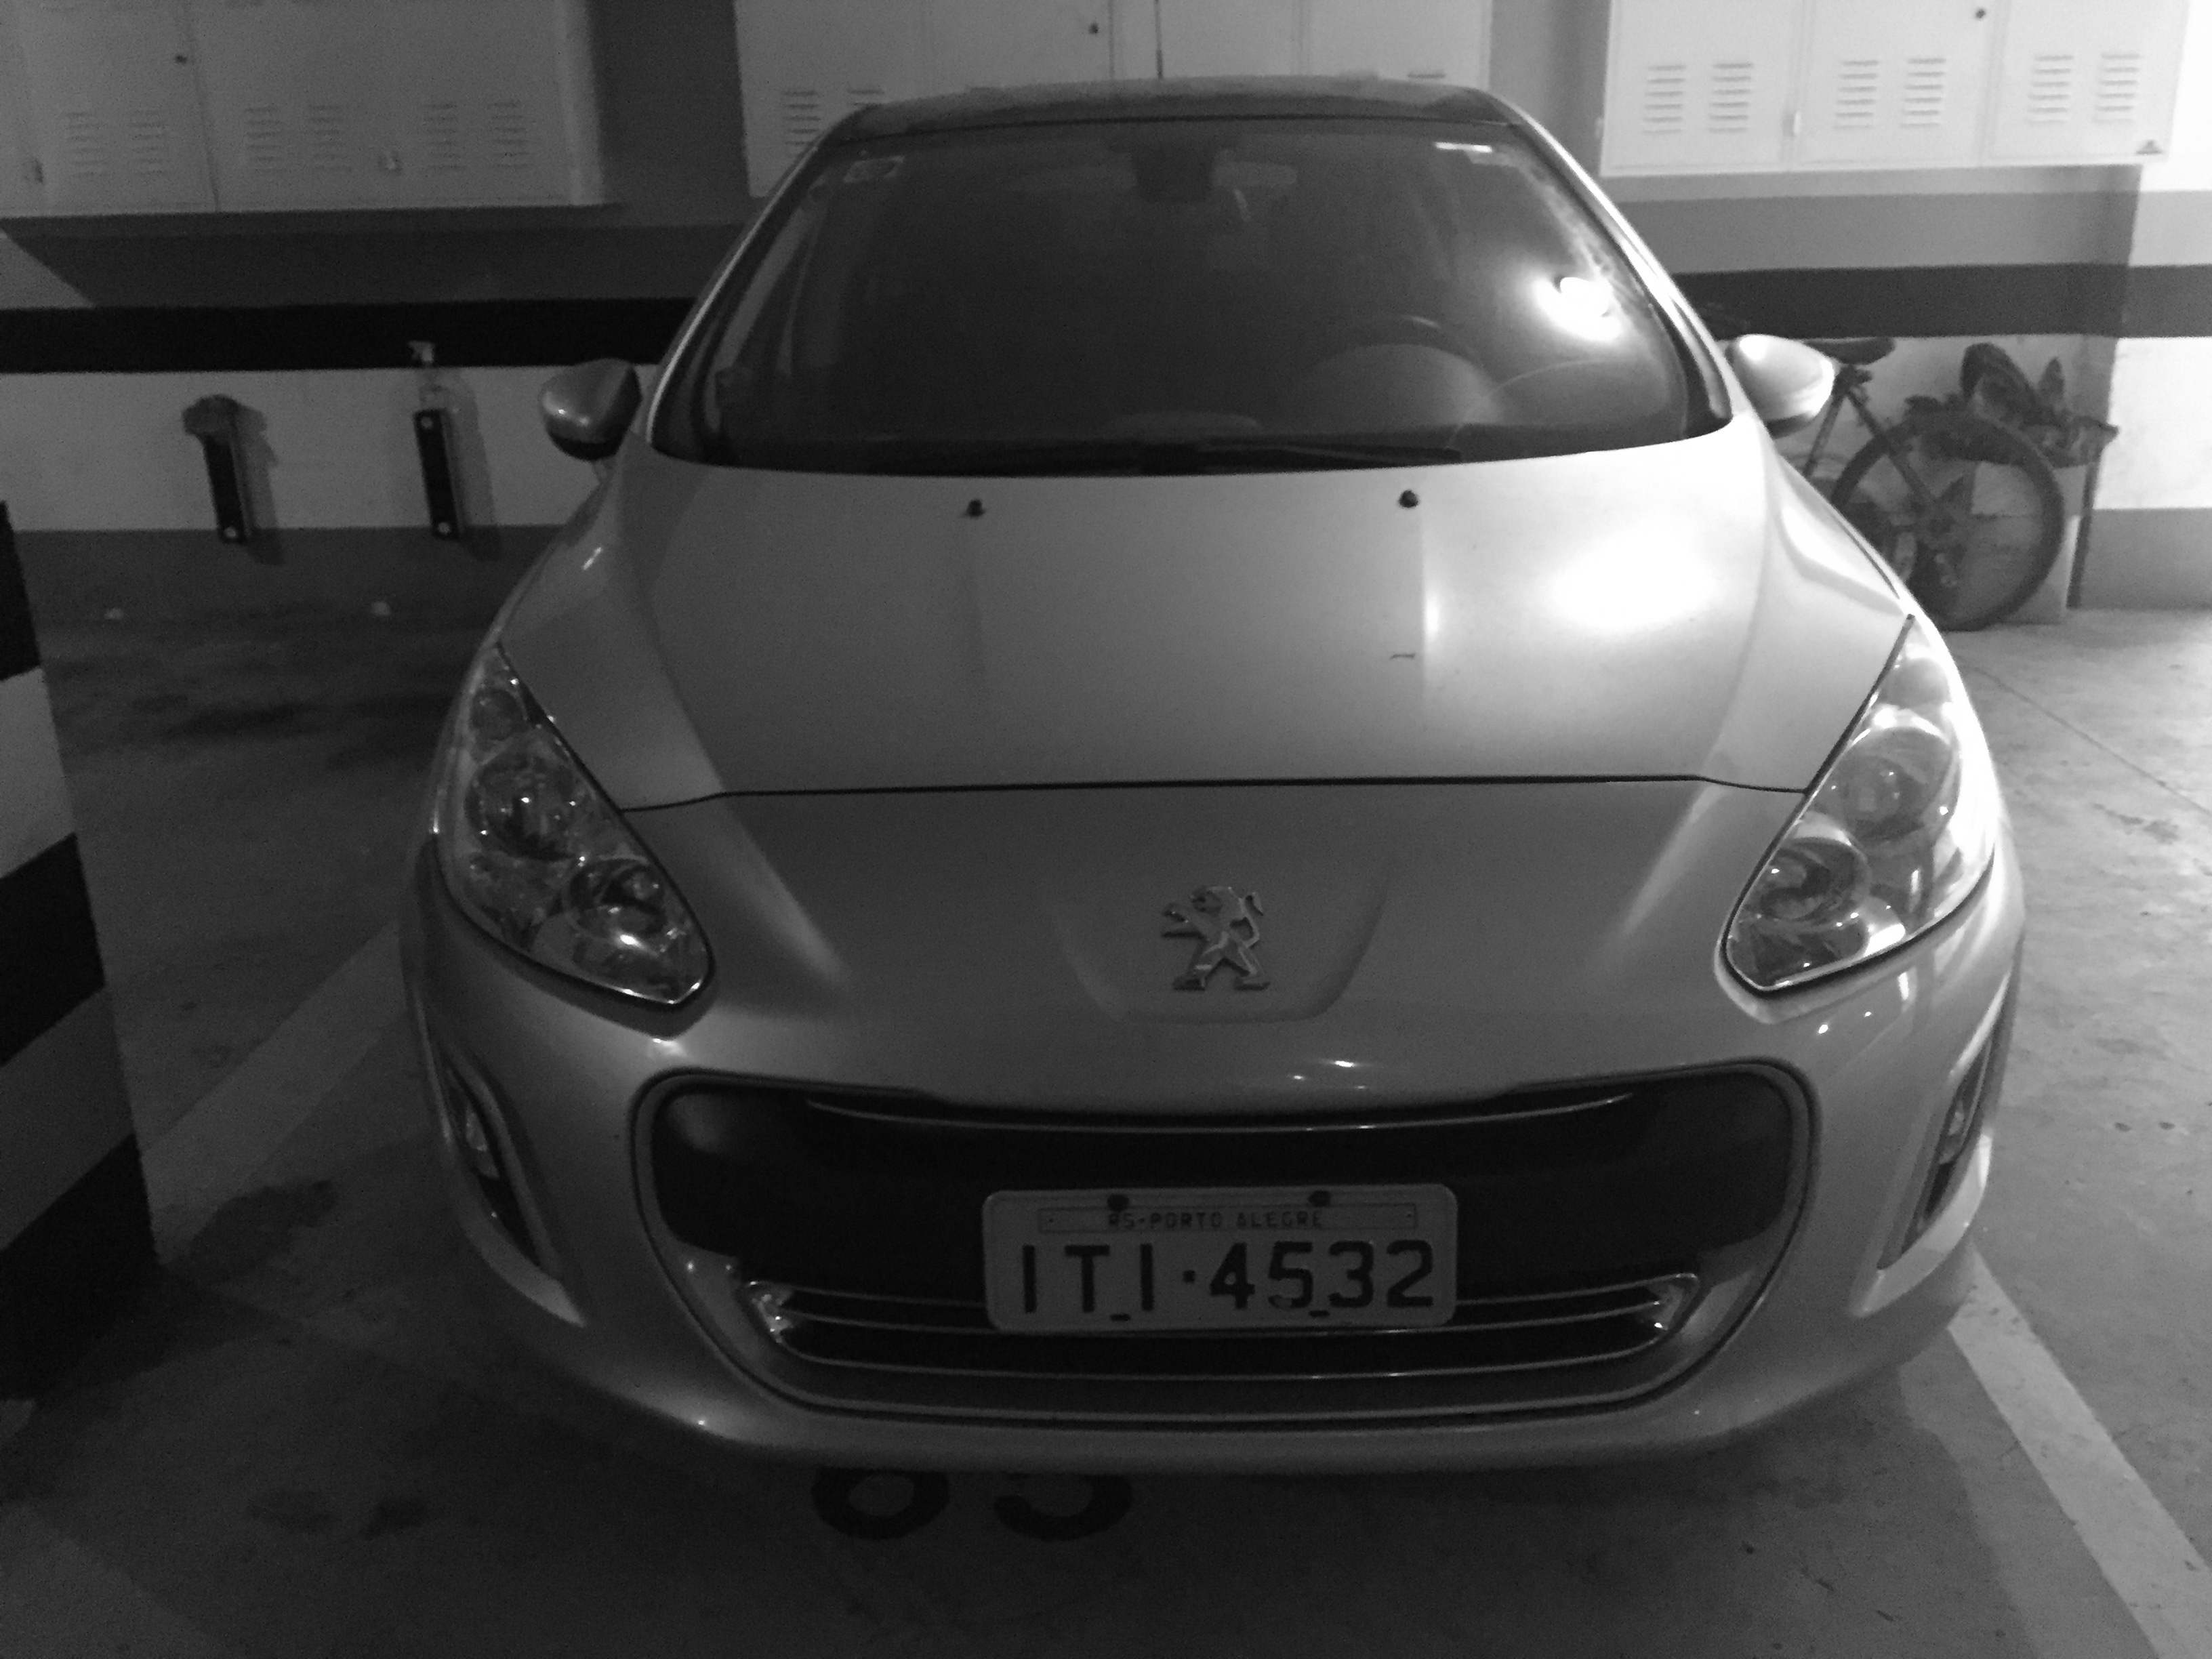
\includegraphics[width=88mm]{peugeotgay.jpg}
	\caption{Veículo que o algoritmo tem dificuldade de reconhecer}
	\label{fig:peugeot_gay}
\end{figure}

\section{Reconhecimento dos caracteres}
\label{sec:reconhecimento_dos_caracteres_resultados}

Inicialmente foi utilizado o \emph{software Tesseract} para fazer o
reconhecimento dos caracteres, mas os resultados utilizando a ferramenta pura
não foram bons. Mesmo limitando os caracteres possíveis, informando ao
\emph{software} se o caractere seria um número ou uma letra, ainda havia
dificuldade no reconhecimento.

Com a substituição do reconhecedor de caracteres \emph{Tesseract} para o
implementado com o algoritmo \emph{K-Nearest Neighbors} os resultados foram bem
melhores, obtendo sucesso no reconhecimento de 86\% das placas extraídas. Até
mesmo em imagens de placas inclinadas, como é o caso da
Figura~\ref{fig:plate_torta_result}, foi possível identificar os caracteres.

\begin{figure}[H]
	\centering
	
\includegraphics[width=88mm]{a42fill_binary_results.jpg}
	\caption{Placa inclinada que o sistema foi capaz de identificar}
	\label{fig:plate_torta_result}
\end{figure}

Das 22 placas extraídas, três delas o reconhecedor de caracteres não teve
capacidade de ler. Dois destes casos foram causados por problemas na imagem e o outro
foi causado por semelhança de caracteres.

Placas com reflexo causado pelo ambiente, como a luz solar, podem impactar no
reconhecimento. O sol refletido no caractere da imagem pode dificultar o
processo de limiarização. Neste processo, ao diferenciar os caracteres escuros
do fundo cinza, a cor do caractere na imagem fica mais clara, sendo ele
parcialmente confundido com fundo. Na figura~\ref{fig:cagado_reflexo} é possível
observar uma placa que o reflexo impediu o reconhecimento correto.

\begin{figure}[H]
	\centering
	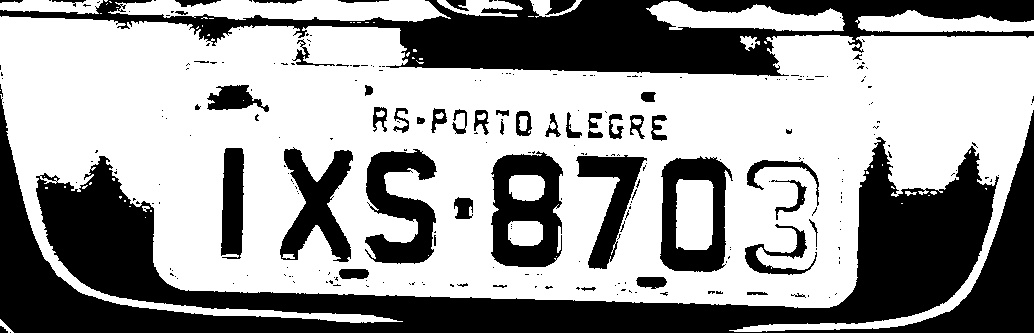
\includegraphics[width=88mm]{3cagado.jpg}
	\caption{Placa com caractere mal reconhecido por causa de reflexo}
	\label{fig:cagado_reflexo}
\end{figure}

Em placas desgastadas, pelo tempo ou pelo carro ter passado por condições climáticas que o degradaram, também houve dificuldade de reconhecimento. Assim como no caso anterior, os caracteres ficaram desfigurados na fase da limiarização, por terem uma variação muito grande nos tons de cinza. Isso faz com que parte do caractere seja confundido com o fundo. Imagem de placa de carro adquirida onde a placa estava desgastada dificultando o reconhecimento pode ser vista na Figura~\ref{fig:placa_desgastada}.

\begin{figure}[H]
	\centering
	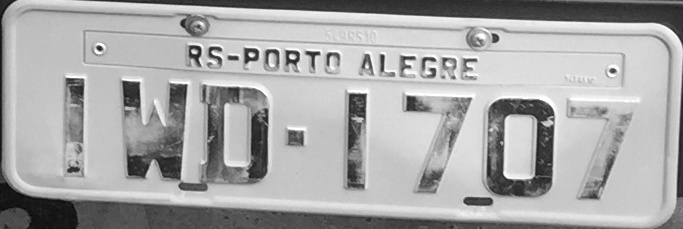
\includegraphics[width=88mm]{plca_desgastada.jpg}
	\caption{Placa desgastada}
	\label{fig:placa_desgastada}
\end{figure}

Somente em um caso, nas imagens de teste adquiridas, ocorreu um erro de reconhecimento de caractere por motivos não causados pelo ambiente ou qualidade da placa. Em uma imagem adquirida com a placa levemente inclinada, houve confusão, por parte do algoritmo, entre os caracteres "O"~e "Q~. Estes caracteres já são bastante semelhantes por si só, mas é possível, também, que o fato de a placa estar inclinada tenha amplificado o erro. A imagem que não foi reconhecida corretamente, ao confundir o "O"~e o "Q", pode ser vista na Figura~\ref{fig:q_confundido_com_o}.

\begin{figure}[H]
	\centering
	
\includegraphics[width=88mm]{q_confundido_com_o.jpg}
	\caption{Placa que confundiu os caracteres O e Q}
	\label{fig:q_confundido_com_o}
\end{figure}

Apesar dos casos em que houve erro, o resultado do reconhecedor de caracteres foi satisfatório. Mesmo tendo sido sido utilizados apenas um exemplo para cada caractere na fase de treinamento, somente em um caso houve confusão no reconhecimento dos caracteres bem segmentados. Com mais exemplos seria possível um reconhecimento ainda mais preciso.

\section{Performance em sistema embarcado}
\label{sec:performance_resultados}

A implementação do algoritmo obteve maus resultados com relação a
performance quando executada como sistema embarcado no \emph{Raspberry Pi}. 
O seu tempo de execução para processar cada imagem foi muito alto, tornando o \emph{software} 
inviável para o uso em casos reais.

Dado o fato de a solução desenvolvida ser dividida em etapas, é possível avaliar
quais os passos levam mais tempo para serem executados, que podem ser
considerados os gargalos da aplicação. Em uma visão mais ampla, fica claro que a
etapa de extração da placa é a que necessita de mais recursos computacionais.
Isso se dá principalmente por ter que processar uma imagem maior que a imagem da
placa. O tempo utilizado para processar a placa extraída é, relativamente, bem
menor.

Para melhor analisar os resultados comparativos, foram calculadas as médias de
tempo de execução de cada etapa em múltiplas imagens e calculados seus valores
percentuais em relação ao tempo total de processamento de uma placa. Esses
valores independem do \emph{hardware} utilizado, permitindo uma visão diferente dos resultados. 
Os resultados comparativos podem ser vistos na Tabela~\ref{tab:resultados_relativos}, as etapas 
estão dispostas na ordem em que são executados pela aplicação. A divisão
das etapas em processos para fazer o \emph{Pipeline} foi feita com base nestes dados.

\begin{table}[H]
\centering
\caption{Resultados relativos da fase de extração}
\label{tab:resultados_relativos}
\begin{tabular}{@{}lr@{}}
\toprule
Etapa                        & Tempo Percentual \\ \midrule
Conversão para tons de cinza & 9\%             \\
Filtro Bilateral             & 22\%             \\
Equalização do Histograma    & 9\%             \\
Limiarização                 & 5\%             \\
Detecção de Bordas           & 10\%             \\
Dilatação                    & 6\%             \\
Preenchimento de espaços     & 5\%             \\
Abertura                     & 16\%             \\
Fechamento                   & 16\%             \\
Extração das Regiões         & 2\%             \\ \bottomrule
\end{tabular}
\end{table}

Ao aplicar o \emph{Pipeline} em múltiplos processos, com o objetivo de
utilizar mais núcleos do processador do \emph{Raspberry Pi}, houve melhora, mas
não muito significativa, no tempo. Por motivos de comparação, foi feito
uma série de testes no \emph{Raspberry Pi} e em um 
\emph{Macbook Pro}, com processador \emph{Intel i7-4770HQ}. Foi avaliado o tempo de processamento
sequencial de uma imagem, o tempo de processamento sequencial, sem utilizar múltiplos processos
de 10 imagens, e o tempo de processamento, utilizando o \emph{Pipeline} de processos
em 10 imagens. Cada um desses testes foi feito 10 vezes e o seu tempo médio foi calculado.
Os resultados podem ser vistos na Tabela XXX.

Em teste com a utilização do módulo de câmera em simulação próxima do real, não foi possível
identificar placas de veículos por causa da performance. As imagens adquiridas ficam muito espaçadas, 
entre um processamento e o outro, e muito raramente consegue-se uma imagem que contenha um carro, deixando
muitos passarem sem identificação.

